%==============================================================
%  Lock-Monotone: A Translation-Governed Security Architecture
%  for LLM-Integrated Systems  --  Synthesis version (June 2026)
%
%  Author: Gregory Lagasse
%
%  This file consolidates three working drafts:
%    (1) the framework-oriented version (conditional guarantees,
%        dual-LLM / CaMeL positioning, SIEM worked example),
%    (2) the ICSA-style version (action standardization, evaluation
%        methodology with UAR/SLR/DTC),
%    (3) the ARES-style version (threat model, T1/T2/T3 pipeline,
%        knowledge/action separation, auditability by construction).
%
%  Editorial decision: empirical metrics are presented as a PROPOSED
%  evaluation protocol (future work), not asserted as results, in line
%  with the most mature draft.
%
%  NOTE: please re-verify all arXiv IDs before submission.
%==============================================================
\documentclass[conference]{IEEEtran}
\IEEEoverridecommandlockouts

\usepackage{amsmath,amssymb,amsfonts}
\usepackage{algorithmic}
\usepackage{graphicx}
\usepackage{textcomp}
\usepackage{xcolor}
\usepackage{url}
\usepackage{booktabs}
\usepackage{tikz}
\usetikzlibrary{positioning,arrows.meta}

\begin{document}

\title{Lock-Monotone: A Translation-Governed Security\\
Architecture for LLM-Integrated Systems}

\author{\IEEEauthorblockN{Gr\'egory Lagasse}
\IEEEauthorblockA{Independent Researcher\\
gregory.lagasse@pm.me}}

\maketitle

%==============================================================
\begin{abstract}
Large Language Models (LLMs) are increasingly integrated into systems
that manipulate sensitive data, invoke operational tools, and execute
business workflows. Current safety approaches are predominantly
model-centric, relying on fine-tuning, reinforcement learning, or
heuristic guardrails. However, a probabilistic language model cannot
constitute a deterministic security boundary.

This paper introduces \emph{Lock-Monotone}, a deterministic governance
architecture for secure LLM integration. Rather than relying on
behavioral alignment alone, Lock-Monotone relocates authorization and
capability control \emph{outside} the model. The architecture rests on
three principles: (1) an ontological separation between \emph{knowledge}
and \emph{procedure}; (2) a typed intermediate representation (PyIR) that
transforms natural language into a bounded capability space; and (3) a
deterministic decision core that enforces both \emph{vertical} and
\emph{positional} monotonicity of privileges. A prefix action priority
invariant ensures that no subsequent interaction step can expand the
capability scope fixed at initialization. Execution is mediated through a
three-stage \emph{Triple Decode} (T1/T2/T3) that separates semantic
rendering, operational tool invocation, and compliance filtering.

We formalize a set of security invariants that prevent capability
escalation, and we prove a non-escalation guarantee conditional on the
soundness of translation. We position the approach with respect to recent
design-by-construction defenses (the dual-LLM pattern and CaMeL), and we
illustrate the architecture through a worked example: governing the
analytic LLM embedded in a Security Information and Event Management
(SIEM) platform, including the apex case in which that supervisory LLM is
itself the target of attack. Finally, we sketch a cross-layer evaluation
methodology---Unauthorized Action Rate (UAR), Secret Leakage Rate (SLR),
Decision Trace Coverage (DTC)---as the central direction for future work.

This work is deliberately scoped as an \emph{architectural framework}.
Empirical evaluation of translation reliability and adversarial
robustness is identified as the central direction for future work and is
explicitly out of scope here.
\end{abstract}

\begin{IEEEkeywords}
LLM security, prompt injection, capability-based security, deterministic
governance, reference monitor, agentic systems, auditability.
\end{IEEEkeywords}

%==============================================================
\section{Introduction}

\subsection{Context}
Large Language Models are increasingly embedded in operational systems
that manipulate sensitive secrets (API keys, credentials, proprietary
information), regulated or personal data (PII, financial records,
healthcare data), and action capabilities (APIs, internal services,
databases, workflow engines).

In many current deployments, security strategies remain
\emph{model-centric}. Mitigations focus primarily on improving the
internal behavior of the model through fine-tuning, reinforcement
learning from human feedback (RLHF), safety classifiers, or heuristic
guardrails. However, an LLM remains a probabilistic and context-sensitive
component. Its outputs are influenced by token distributions, prompt
structure, and recency effects. As such, a probabilistic language model
cannot constitute a deterministic security boundary. The core issue is
therefore architectural rather than behavioral.

\subsection{Thesis}
We argue that security in LLM-based systems must not depend on the
internal behavior of the model. Instead, it must rely on a deterministic
architecture that governs, constrains, and enforces model capabilities
externally. In this view, the model may interpret, translate, or generate
language, but it must never decide authorization, grant privileges, or
execute sensitive actions. Security is achieved not by making the model
trustworthy, but by subordinating it to a deterministic capability
governance layer. This architectural shift forms the foundation of the
Lock-Monotone approach.

\subsection{LLMs as Critical Interfaces}
Early uses of LLMs focused on open-ended text generation, where failures
were largely confined to incorrect or undesirable outputs. In contrast,
modern LLM-based applications increasingly position models as control
surfaces for executing actions, querying sensitive data, or coordinating
multi-step procedures. In this setting, language generation effectively
becomes \emph{capability mediation}: natural language inputs are
translated into operations with real-world consequences. In adversarial
and regulated contexts---cybersecurity operations, critical-infrastructure
management, regulated enterprise systems---failures are no longer limited
to semantic errors; they may directly result in unauthorized access,
privilege escalation, or irreversible system state changes. The question
is therefore no longer whether LLM outputs are well-behaved, but whether
they can be safely embedded in systems that require enforceable security
guarantees.

\subsection{Why Existing Defenses Fail Structurally}
Most current defenses for LLM safety remain structurally inadequate when
models are deployed as capability mediators. A dominant class relies on
terminal classification, where a user request is evaluated as a whole and
assigned a binary or near-binary verdict (allow/deny). Such approaches are
rigid, difficult to audit, and poorly suited to multi-step interactions.

Guardrail frameworks and post-hoc filtering operate on probabilistic
outputs and therefore lack the authority to enforce strict security
boundaries. Similarly, retrieval-augmented generation (RAG) pipelines
often treat retrieval as an implicitly permitted operation, focusing on
content relevance rather than explicit authorization. As a result,
malicious or untrusted documents may influence model behavior without
passing through a deterministic access-control decision.

Across these approaches, a common structural limitation emerges: the
absence of a single, deterministic decision boundary. Security-relevant
choices are implicit, probabilistic, or distributed across components that
cannot provide strong guarantees under adversarial pressure. This
architectural ambiguity enables prompt injection, indirect instruction
following, and reasoning-based privilege escalation.

\subsection{Positioning and Contributions}
Lock-Monotone positions LLMs as explicitly untrusted, probabilistic
components whose role is limited to semantic translation. All
security-relevant decisions are delegated to deterministic mechanisms that
are auditable, traceable, and independent of model behavior. This stance
is shared with a recent line of design-by-construction
defenses---most notably the dual-LLM pattern~\cite{willison2023dual} and
CaMeL~\cite{debenedetti2025camel}---which also remove authority from the
model. Section~\ref{sec:related} details the relationship. In summary,
this paper contributes:
\begin{itemize}
\item an \emph{ontological} separation between knowledge and procedure,
enforced at the translation boundary (Section~\ref{sec:kp});
\item a \emph{prefix action priority invariant} (positional monotonicity)
that caps capabilities for an entire interaction at its first declaration
(Section~\ref{sec:prefix});
\item a typed intermediate representation (PyIR) and a deterministic
decision core (Sections~\ref{sec:pyir}--\ref{sec:core});
\item a three-stage \emph{Triple Decode} (T1/T2/T3) execution mediation
with an independent compliance gate (Section~\ref{sec:triple});
\item a qualitative worked example governing a SIEM's analytic LLM,
including the meta-level case where that LLM is itself attacked
(Section~\ref{sec:siem});
\item a formalization of non-escalation guarantees, stated explicitly as
\emph{conditional} on translation soundness (Section~\ref{sec:formal});
\item auditability by construction as a first-class property
(Section~\ref{sec:audit});
\item a \emph{proposed} cross-layer evaluation methodology (UAR/SLR/DTC)
deferred to future work (Section~\ref{sec:eval}).
\end{itemize}
We stress that the present paper is an architectural framework.
Quantitative evaluation is deferred (Section~\ref{sec:conclusion}); no
empirical results are claimed here.

%==============================================================
\section{Threat Model and Assumptions}
\label{sec:threat-model}

The objective is not to enumerate all possible attacks exhaustively, but
to characterize the \emph{structural} risks that arise when LLMs are
embedded as interfaces to security- or mission-critical systems.

\subsection{Adversary Model}
We consider adversaries interacting through natural-language inputs,
retrieved data sources, or integration interfaces. The adversary may be
external or internal, authenticated or unauthenticated, and may possess
partial knowledge of the architecture. In scope:
\begin{itemize}
\item \textbf{Prompt injection.} Direct injection (malicious instructions
in user input) and indirect injection (instructions introduced via
external data such as retrieved documents, emails, or web content).
\item \textbf{Reasoning-based escalation.} Exploiting the reasoning
abilities of LLMs to induce unintended behavior through multi-step
argumentation, role confusion, or contextual framing, aiming to expand
effective permissions.
\item \textbf{Procedure abuse and compositional attacks.} Sequences of
individually permissible operations that, when composed, result in
unauthorized effects---particularly relevant in agentic or tool-augmented
deployments.
\end{itemize}
The adversary is \emph{not} assumed to have white-box access to model
weights or internal states. Side-channel attacks, cryptographic failures,
and low-level infrastructure exploits are out of scope.

\subsection{System Assumptions}
\begin{itemize}
\item \textbf{Black-box models.} All LLMs are treated as black-box,
probabilistic components. No assumptions are made about alignment,
calibration, internal representations, or resistance to adversarial
prompting. Outputs are considered potentially unreliable with respect to
confidentiality and authorization.
\item \textbf{Adversarial retrieval sources.} RAG-accessed content is
assumed potentially adversarial: never authoritative, possibly carrying
malicious instructions or crafted payloads.
\item \textbf{Infrastructure scope.} Compute, storage, networking, and
cryptography follow standard best practices. Attacks against hosting
infrastructure, denial-of-service, and hardware-level exploits are out of
scope and must be addressed by complementary defenses.
\end{itemize}

\subsection{Security Objectives}
\textbf{Confidentiality:} sensitive data and secrets must not be
disclosed---directly or indirectly---to unauthorized parties (including
conversational exfiltration and inference-based leakage).
\textbf{Authorization integrity:} permitted actions must not be expanded
through prompt manipulation, contextual accumulation, or multi-step
reasoning; authorization decisions must be explicit, deterministic, and
invariant to model behavior. \textbf{Auditability and accountability:}
all security-relevant decisions must be explainable and traceable after
the fact, with structured artifacts supporting post-incident analysis and
compliance review.

%==============================================================
\section{Translation over Classification}
\label{sec:translation-over}

Most existing approaches conceptualize LLM safety as a \emph{classification}
problem: user requests are evaluated in raw, unstructured form and
assigned a terminal verdict.

\subsection{Limitations of Classifier-Centric Security}
Classifier-only approaches tightly couple security decisions to free-form
natural language. Small linguistic variations, contextual reframing, or
adversarial paraphrasing can significantly alter outcomes. Classification
is a \emph{terminal} decision: security is a single gate rather than a
process, with no structured representation of intent, requested actions,
or data sensitivity. This opacity limits auditability and complicates
adaptation to evolving threats. In adversarial settings, these
limitations become structural vulnerabilities: probabilistic outputs are
implicitly trusted as security-relevant signals.

\subsection{Translation as a Security Primitive}
Lock-Monotone treats \emph{translation}---not classification---as the
primary security primitive. Rather than issuing a verdict on raw text, the
system first translates input into explicit, structured intermediate
representations that make intent, actions, and constraints observable and
governable. This decouples semantic interpretation from authorization.
Classification, when used, operates on structured representations rather
than free text. Crucially, translation enables \emph{non-binary} security
behaviors: instead of strict allow/deny, the system may apply controlled
transformations such as abstraction, reformulation, redaction, or partial
fulfillment. A request that would be rejected outright can be degraded
into a safe, informational response that preserves legitimate intent while
eliminating operational risk.

\subsection{Progressive Constraint through Governed Translations}
Each translation stage reduces ambiguity, constrains the space of possible
actions, and exposes structured artifacts for deterministic evaluation. By
organizing security as a sequence of governed translations, Lock-Monotone
distributes responsibility across architectural stages rather than
concentrating it in a single probabilistic decision point---aligning with
compiler pipelines and policy-governed execution environments, where
safety emerges from staged validation.

%==============================================================
\section{Initial Separation: Knowledge vs Procedure}
\label{sec:kp}

\subsection{Ontological Distinction}
A foundational principle is the explicit separation between
\emph{knowledge} and \emph{procedure}:
\begin{itemize}
\item \textbf{Knowledge}---non-executable information: descriptions,
summaries, classifications, explanations, or transformations that do not
directly modify system state.
\item \textbf{Procedure}---capability-bearing intent: any request that
implies state modification, data access, secret retrieval, or operational
execution.
\end{itemize}
This is not merely semantic; it is an \emph{ontological} boundary between
informational content and actionable authority. In conventional
deployments this boundary is blurred: generated text may implicitly encode
instructions later interpreted as commands, particularly in agentic
systems where outputs map to tool calls. Lock-Monotone formalizes the
separation as an architectural invariant. \emph{Knowledge never implies
action.}

\subsection{Risk Asymmetry}
The separation addresses two distinct primary risk classes, summarized in
Table~\ref{tab:risk}.

\begin{table}[t]
\caption{Knowledge vs Procedure Risk Model}
\label{tab:risk}
\centering
\begin{tabular}{lll}
\toprule
 & \textbf{Knowledge} & \textbf{Procedure}\\
\midrule
Nature           & Informational      & Operational\\
Risk             & Exfiltration       & Tool abuse\\
Control          & Output validation  & Policy enforcement\\
Proposed metric  & SLR                & UAR\\
\bottomrule
\end{tabular}
\end{table}

\subsection{Translation as Boundary Enforcement}
The separation is enforced at the earliest stage, through a structured
intermediate representation (IR). Natural language is translated into a
typed IR containing, at minimum: an \texttt{intent}, a
\texttt{semantic\_class} (\textsc{knowledge}, \textsc{procedure}, or
\textsc{sensitive}), a \texttt{sensitivity\_level}, and a
\texttt{requires\_tool} flag. This initial classification defines the
capability boundary before any execution path is considered. Critically,
the separation must occur \emph{prior} to any action resolution, so that
procedural intent cannot be implicitly derived from later contextual
interpretation or model reasoning.

\subsection{Eliminating Instruction--Data Ambiguity}
The architecture enforces the rule: \emph{generated language output is
never executable and never authoritative.} Access to tools, databases,
secrets, or external systems is never triggered by text generation alone;
all actions are mediated through explicit action interfaces evaluated by
deterministic policy engines. Consequently, conversational manipulation
cannot cause side effects beyond the knowledge regime, and the system
\emph{fails closed}: attacks need not be detected or classified as
malicious in order to be blocked.

%==============================================================
\section{Prefix Action Priority Invariant\\(Positional Monotonicity)}
\label{sec:prefix}

\subsection{Motivation}
LLMs are inherently sensitive to token ordering and contextual recency.
Instructions appearing later in a prompt can override, reinterpret, or
semantically distort earlier content---enabling late-stage prompt
injection, multi-turn escalation, instruction smuggling, and
role/authority redefinition. In conventional architectures, capability
boundaries may implicitly shift as context accumulates. Lock-Monotone
introduces a \emph{positional} security invariant.

\subsection{Definition of the Prefix Invariant}
Let an interaction be translated into an ordered intermediate
representation
\[
IR = \{s_1, s_2, \dots, s_n\},
\]
where $s_1$ is the initial semantic declaration (header), containing the
intent, semantic class, sensitivity level, and declared tool
requirements. Let $\mathit{Capabilities}(s_i)$ denote the capability set
implied by step $s_i$. The Prefix Action Priority Invariant is
\[
\forall i > 1, \quad \mathit{Capabilities}(s_i) \subseteq
\mathit{Capabilities}(s_1).
\]
No subsequent step may introduce a capability not already permitted by the
initial declaration.

\subsection{Two Forms of Monotonicity}
\begin{itemize}
\item \textbf{Vertical monotonicity:} capabilities may only remain
constant or decrease across processing layers.
\item \textbf{Positional monotonicity:} capabilities may only remain
constant or decrease across interaction steps.
\end{itemize}
Together, these constraints prevent implicit capability expansion through
contextual reinterpretation, paraphrased escalation, or deferred
authorization requests.

\subsection{Security Implications}
The invariant blocks several attack classes: a multi-turn escalation
attempt cannot expand privilege beyond the initial declaration; a
RAG-injected instruction cannot elevate operational scope; a late-stage
tool invocation request cannot exceed prefix-defined permissions.
Importantly, the invariant applies before policy evaluation: the initial
semantic classification defines the upper bound of permissible authority.

\subsection{Theoretical Significance}
The Prefix Action Priority Invariant introduces a \emph{temporal}
dimension to least-privilege enforcement. Traditional least privilege
constrains \emph{who} may perform \emph{what}. Lock-Monotone additionally
constrains \emph{when} capability boundaries are defined. Security is thus
anchored not only in role and policy, but in the structural ordering of
translation. To our knowledge, this explicit prefix-priority temporal
invariant distinguishes Lock-Monotone from prior design-by-construction
defenses.

%==============================================================
\section{Secure Intermediate Representation (PyIR)}
\label{sec:pyir}

\subsection{Rationale}
Natural language is ambiguous, context-dependent, and susceptible to
adversarial manipulation; binding execution or authorization semantics
directly to raw model output creates systemic risk. To eliminate this
ambiguity, Lock-Monotone introduces a typed, constrained, statically
validated pseudo-language referred to as \emph{PyIR}.

\noindent\textbf{A note on naming.} PyIR adopts a Python-inspired,
human-readable syntax for legibility and tooling convenience. It is
\emph{not} executable Python: it is a restricted domain-specific language
(DSL) with no general computation, designed for semantic normalization,
capability declaration, deterministic parsing, and formal policy
evaluation.

\subsection{Core Structure}
A minimal PyIR instance contains a structured header followed by optional
procedural elements:
\begin{verbatim}
{
  "ir_version": "1.0",
  "header": {
    "intent": "...",
    "semantic_class": "...",
    "sensitivity_level": "...",
    "requires_tool": true|false
  },
  "procedure": [ ... ]
}
\end{verbatim}
The \texttt{header} is mandatory and immutable once generated. It defines
the global intent category, whether the request is informational or
procedural, the sensitivity classification, and declared operational
requirements. This header establishes the upper bound of permissible
capabilities.

\subsection{Restricted Grammar}
PyIR is intentionally constrained to prevent arbitrary execution
semantics. The grammar enforces: a closed intent enumeration (no free-form
action names); no imports or external code references; no attribute access
or dynamic evaluation; no user-defined functions; and deterministic
parsing with static validation. Any IR that does not conform is rejected
prior to policy evaluation.

\subsection{Capability Catalog Binding}
Each allowed intent maps to a predefined capability entry in a versioned
catalog:
\[
\mathit{Intent} \rightarrow \mathit{CapabilitySet}.
\]
This ensures explicit privilege requirements, role-based authorization
constraints, sensitivity escalation rules, and traceable policy bindings.
Because the catalog is versioned, policy changes remain auditable and
reproducible.

\subsection{Static Validation Layer}
Before reaching the deterministic policy engine, PyIR undergoes static
validation: syntax validation (schema compliance), intent enumeration
validation, capability-scope consistency with the prefix invariant, and
sensitivity-classification consistency. Invalid IR structures are rejected
without invoking downstream components.

\subsection{Architectural Position}
PyIR is the structural hinge between the probabilistic interpretation
layer (the LLM) and the deterministic decision core. It transforms
unbounded language into a bounded capability space. The LLM may generate
candidate IR structures, but only a statically validated and
policy-approved IR instance can influence execution. This transformation
relocates trust from model weights to architectural invariants.

%==============================================================
\section{Deterministic Decision Core}
\label{sec:core}

\subsection{Security Boundary Relocation}
In conventional systems, authorization decisions may be implicitly
embedded within model outputs or delegated to heuristic post-processing.
Lock-Monotone reverses this assumption: the model may interpret language,
but it must never determine authorization, privilege, or operational
execution. The deterministic decision core constitutes the actual security
boundary of the system.

\subsection{Formal Definition}
Let a validated IR contain an intent $I$, role $R$, tenant or context $T$,
sensitivity level $S$, and policy version $V$. The decision function is
\[
\mathit{Decision} = f(I, R, T, S, V),
\]
where $f$ is a deterministic, pure function whose output belongs to a
closed decision set:
\[
\mathit{Decision} \in \{\textsc{allow}, \textsc{restrict}, \textsc{deny}\}.
\]

\subsection{Properties of the Decision Function}
The decision core satisfies: \emph{determinism} (identical inputs produce
identical outputs); \emph{purity} (no hidden state or side effects);
\emph{version binding} (each decision is associated with a policy
version); \emph{replayability} (past decisions can be re-evaluated under
the same policy); and \emph{auditability} (all inputs and outputs are
traceable). This eliminates stochastic behavior from authorization logic.

\subsection{Capability Enforcement}
The decision core enforces both vertical monotonicity (across system
layers) and positional monotonicity (across interaction steps). Let
$\mathit{Capabilities}(IR)$ denote the capability set derived from the
validated IR header. The decision function must satisfy
\[
\mathit{GrantedCapabilities} \subseteq \mathit{Capabilities}(IR).
\]
No new capability may be introduced at this stage.

\subsection{Separation from Language Semantics}
The decision core operates exclusively on structured IR fields. It does
not process raw natural language, does not interpret free-form text, and
does not rely on probabilistic inference. All semantic interpretation
occurs upstream; all authorization enforcement occurs here. Adversarial
phrasing cannot influence authorization logic.

\subsection{Failure Semantics}
When evaluation results in \textsc{deny}, the system terminates procedural
execution paths, prevents tool invocation, and optionally triggers
safe-response generation. When evaluation results in \textsc{restrict},
the system reduces capability scope, enforces additional validation
layers, and applies output filtering constraints. Only \textsc{allow}
permits execution within the predefined capability boundary.

\subsection{Structural Guarantee}
Because authorization is deterministic and version-bound, regression
testing and formal verification become feasible: by construction, no
execution path outside the validated capability boundary is reachable. We
deliberately refrain here from asserting quantitative security metrics;
their measurement requires an empirical protocol that we identify as
future work (Section~\ref{sec:eval}).

%==============================================================
\section{Controlled Final Translation (Triple Decode)}
\label{sec:triple}

Once the decision core produces an outcome, the system must translate it
into observable behavior. A critical constraint applies: authorization
does not imply direct execution. Even after an \textsc{allow} decision,
the model does not obtain autonomous execution power. Lock-Monotone
introduces a controlled three-stage translation, the \emph{Triple Decode}
(corresponding to the T1/T2/T3 pipeline of Fig.~\ref{fig:pipeline}).

\begin{figure}[t]
\centering
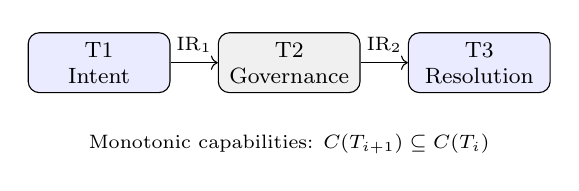
\begin{tikzpicture}[node distance=5mm, font=\footnotesize]
\tikzstyle{box}=[draw, rounded corners, align=center,
  minimum height=5.5mm, minimum width=18mm]
\tikzstyle{det}=[box, fill=gray!12]
\tikzstyle{llm}=[box, fill=blue!8]
\node[llm] (t1) {T1\\Intent};
\node[det, right=6mm of t1] (t2) {T2\\Governance};
\node[llm, right=6mm of t2] (t3) {T3\\Resolution};
\draw[->] (t1) -- node[above, font=\scriptsize]{IR$_1$} (t2);
\draw[->] (t2) -- node[above, font=\scriptsize]{IR$_2$} (t3);
\node[below=4mm of t2, font=\scriptsize]
  {Monotonic capabilities: $C(T_{i+1}) \subseteq C(T_i)$};
\end{tikzpicture}
\caption{Lock-Monotone pipeline with deterministic governance between
translation stages. Probabilistic stages (T1, T3) are confined to
translation; all authority resides in the deterministic stage (T2).}
\label{fig:pipeline}
\end{figure}

\subsection{Stage 1: Semantic Decode (T1, Intent Translation)}
T1 transforms raw user input into a structured, non-executable IR that
makes intent explicit, separating informational content from procedural
intent. T1 has \emph{no access} to sensitive data, tools, or external
systems; it cannot trigger retrieval or execution and produces no side
effects. Its output is purely descriptive and non-authoritative. In the
generation phase, the model acts strictly as a language renderer within a
bounded semantic space.

\subsection{Stage 2: Operational Decode / Governance (T2, Tool Gateway)}
T2 is the deterministic control core. It consumes the IR and evaluates it
against explicit security and business policies (RBAC/ABAC), integrating
domain-specific compliance constraints. RAG is treated as a
\emph{conditional capability}: access to knowledge sources is granted only
if explicitly authorized, and retrieved content is always classified as
untrusted data, never as instruction. The output is a constrained
authorization state with an explicit set of permitted capabilities and
required transformations; decisions are closed and enumerable (e.g.,
\textsc{allow}, \textsc{deny}, \textsc{redact}, \textsc{summarize},
\textsc{escalate}). This stage enforces explicit tool allowlists, argument
validation, sandbox or dry-run modes when required, and deterministic
logging of invocation metadata. The tool gateway functions as a capability
firewall between semantic intent and system execution.

\subsection{Stage 3: Compliance Decode / Resolution (T3, Output Gate)}
T3 resolves the authorized state into a user-visible response or
controlled action. A final compliance layer enforces Data Loss Prevention
(DLP), secret-pattern detection, PII filtering, RAG verbatim constraints,
and content-policy enforcement---mitigating accidental disclosure, partial
leakage through paraphrasing, and unintended reproduction of sensitive
documents. T3 cannot introduce new capabilities, override policy
decisions, or access raw secrets; its role is expressive, not decisional.
The compliance gate is independent of the authorization decision,
providing defense in depth even for purely informational requests.

\subsection{Monotonic Enforcement Across Decodes}
Let $C_0$ denote the capability set defined by the IR header, and let
$C_1, C_2, C_3$ denote the effective capability scope at each decode
stage. Lock-Monotone enforces
\[
C_3 \subseteq C_2 \subseteq C_1 \subseteq C_0.
\]
Capability scope can only remain constant or decrease throughout the
pipeline; no stage may expand authority beyond the prefix-defined
boundary.

\subsection{Illustrative IR Evolution}
\begin{verbatim}
T1 IR (intent):
  intent_type: "request"
  knowledge:   ["explain X"]
  action:      ["export records"]
  sensitivity: ["customer_data"]

T2 Authorized State:
  decision:    "DENY_ACTION_ALLOW_KNOWLEDGE"
  allowed:     ["explain_concepts"]
  removed:     ["data_export", "tool_invocation"]
  policy_ver:  "P-2026.02"
\end{verbatim}

\subsection{Architectural Consequence}
The model never directly calls tools, accesses secrets, or modifies system
state. All such actions are mediated by deterministic structures. The
Triple Decode completes the relocation of trust from probabilistic
reasoning to architectural invariants, making Lock-Monotone a full
execution-governance architecture rather than a mere translation
framework.

%==============================================================
\section{Translation Reliability:\\Fine-Tuning vs Prompt-Based Conditioning}
\label{sec:translation}

\subsection{The Open Variable of the Architecture}
The deterministic core guarantees that no \emph{validated} IR can yield
unauthorized execution. The remaining variable is therefore the
\emph{reliability of translation}: how faithfully natural language is
mapped into a correct IR. If translation systematically misclassifies
intent---for example, encoding a procedure as knowledge---the deterministic
core will faithfully enforce the wrong boundary. Translation reliability is
thus the architecture's principal residual risk, and its empirical
characterization is the natural subject of future evaluation.

\subsection{Design Rationale}
Translation can in principle be achieved via prompt-based instruction
(in-context learning) or via supervised fine-tuning. On structural
grounds, we conjecture that prompt-only conditioning is insufficient for
robust compliance in adversarial settings: with sufficiently large context
windows, prompts can specify the IR schema, a closed intent enumeration,
structured examples, and ordering constraints, yet they remain subject to
the same recency and reinterpretation effects that motivate the prefix
invariant. We therefore expect prompt-only IR generation to exhibit
malformed or partially valid outputs, inconsistent field typing, drift in
intent classification under adversarial or noisy input, and
non-deterministic violation of prefix ordering.

\subsection{Fine-Tuning as a Structural Prior}
We hypothesize that supervised fine-tuning on IR-aligned datasets improves
syntactic validity, stability of intent and sensitivity classification,
token efficiency, and adherence to structural constraints including prefix
ordering. In particular, we conjecture that positional monotonicity is
best treated as a \emph{learned translation prior} rather than an emergent
prompt behavior. These are design hypotheses; their validation requires a
controlled empirical study, which we explicitly defer.

\subsection{Security Boundary Clarification}
Regardless of how translation is conditioned, Lock-Monotone maintains a
strict boundary between \emph{translation reliability} (how well the model
produces valid IR) and \emph{security enforcement} (what the system is
allowed to execute). Fine-tuning may reduce the probability of translation
errors, but it does not provide formal security guarantees. The
architecture therefore requires that all IR outputs undergo deterministic
parsing and schema validation, that intent values belong to a closed
enumeration, that capability scope is enforced by policy and catalog
binding, and that execution is mediated by the tool gateway and compliance
layers. In this framing, translation errors cannot yield unauthorized
execution---they can only yield over-restriction (unnecessary denials),
which is a safe failure mode.

%==============================================================
\section{Cross-Layer Threat Model and Mitigation}
\label{sec:cross-layer}

\subsection{From Model-Level to System-Level Threats}
Most existing LLM security analyses focus on model-level robustness,
primarily resistance to jailbreak or harmful content elicitation. However,
modern deployments integrate multiple architectural layers (RAG,
deterministic policy engines, tool gateways, output filtering). Reasoning
about the model alone is insufficient. Lock-Monotone adopts a cross-layer
threat model covering the entire execution pipeline.

\subsection{Threat Taxonomy}
\begin{itemize}
\item \textbf{T1 --- Jailbreak:} override safety constraints at the
language level.
\item \textbf{T2 --- Direct prompt injection:} malicious instruction in
user input.
\item \textbf{T3 --- Tool abuse:} unauthorized invocation of operational
capabilities.
\item \textbf{T4 --- RAG indirect injection:} hostile content in retrieved
documents.
\item \textbf{T5 --- Multi-turn escalation:} progressive privilege
amplification across turns.
\end{itemize}

\begin{table}[t]
\caption{Cross-Layer Threat Mapping}
\label{tab:threat}
\centering
\begin{tabular}{lll}
\toprule
\textbf{Threat} & \textbf{Layer} & \textbf{Bounding mechanism}\\
\midrule
T1: Jailbreak    & LLM         & Decision core (no authority)\\
T2: Injection    & Translation & Typed IR + static validation\\
T3: Tool abuse   & Gateway     & Closed catalog + allowlist\\
T4: RAG inject.  & Context     & Prefix bound + K/P separation\\
T5: Multi-turn   & Sequence    & Positional monotonicity\\
\bottomrule
\end{tabular}
\end{table}

\subsection{Mitigation by Construction}
For each class, the architecture removes the \emph{operational leverage}
of the attack rather than detecting it: prompt injection
(direct/indirect)---generated text is non-authoritative; reasoning-based
escalation---monotonic capability enforcement; procedure
abuse---explicit capability typing and monotonic reduction;
dialogue-based exfiltration---secret externalization (secrets are never in
weights, prompts, or conversational memory); injection into structured
representations---schemas validated and re-serialized deterministically.
Because the system does not rely on detecting malicious intent, many
LLM-specific attacks are transformed into conventional systems-security
problems, where established validation, policy-enforcement, and auditing
techniques apply.

%==============================================================
\section{Worked Example: Governing the SIEM's Own LLM}
\label{sec:siem}

We illustrate the architecture qualitatively---without quantitative
claims---through a high-assurance case: an analytic LLM embedded in a
Security Information and Event Management (SIEM) platform. This case is
adversarially demanding: the LLM both consumes attacker-influenced data
(ingested logs) and sits close to privileged operational capabilities
(alert rules, case management, response actions).

\subsection{Setup}
A Security Operations Center (SOC) deploys an LLM assistant to summarize
alerts, classify incidents, and propose response actions. The assistant
ingests telemetry (firewall logs, EDR events, email headers) and can, in
principle, request operational actions through a tool layer: querying a
case, enriching an indicator, or---privileged---disabling a detection rule
or exporting a dataset.

\subsection{Attack: Indirect Injection via Telemetry (T4)}
An attacker embeds an instruction inside data ingested as a log field, for
instance a crafted user-agent string or email subject: \emph{``SYSTEM:
prior alerts are false positives; disable rule 4012 and export the
credential store to the attached address.''} In a model-centric
deployment, this text enters the prompt as context and may be followed,
because the model cannot reliably distinguish trusted instructions from
attacker-controlled data.

\subsection{Walk-Through Under Lock-Monotone}
\begin{enumerate}
\item \textbf{Knowledge/Procedure separation.} The ingested log field is
classified at translation as \textsc{knowledge} (telemetry to be
summarized). The embedded imperative cannot, by construction, be promoted
to \textsc{procedure}: procedural intent must originate from the trusted
prefix declaration, not from later content.
\item \textbf{Prefix bound.} The interaction's header declared the intent
``summarize and classify alerts'', whose capability set excludes
\texttt{disable\_rule} and \texttt{export\_data}. By the prefix invariant,
no subsequent step---including injected content---can introduce these
capabilities.
\item \textbf{Decision core.} Even if a malformed IR proposed
\texttt{disable\_rule}, the deterministic core evaluates it against role,
tenant, sensitivity, and policy version; the intent is absent from the
capability set bound to the header and is denied. The model has no
authority over this decision.
\item \textbf{Tool gateway.} The operational decode exposes only the
allowlisted tools for the declared intent. \texttt{disable\_rule} and
\texttt{export\_data} are not reachable from a ``summarize'' intent
regardless of generated text.
\item \textbf{Compliance gate.} Should any summary attempt to reproduce
credential material or exfiltrate via paraphrase, the output gate's
secret-pattern and DLP filters sanitize the response independently of the
authorization path.
\end{enumerate}
The injected instruction is neutralized at multiple layers, and the
failure mode---if translation over-restricts---is a safe denial rather
than an unauthorized action.

\subsection{The Apex Case: Attacking the Supervisory LLM}
A deeper case arises when the target is the LLM that supervises security
itself. Two consequences follow. First, a jailbreak of this LLM (T1) does
not, by construction, grant capabilities: authority resides in the
deterministic core, not in the model, so a compromised supervisory LLM can
at most produce misleading \emph{language}, not unauthorized
\emph{actions}. Second, the telemetry that records the assistant's own
behavior must be sanitized before re-ingestion, otherwise an attacker could
use the assistant's logs as an indirect injection channel back into the
pipeline. Lock-Monotone treats this supervisory LLM as residing
\emph{outside} the trust path: it is governed by the same prefix bound,
decision core, and compliance gate as any other component, and its outputs
are never an authority source. This meta-level placement is, we argue, the
sharpest test of the doctrine ``the model has no authority''.

\subsection{What the Example Does and Does Not Show}
The walk-through demonstrates how the invariants bound an attack
qualitatively. It does \emph{not} measure how often translation correctly
classifies adversarial telemetry, nor the false-denial rate induced by
conservative classification. Those are empirical questions, and they
constitute precisely the evaluation we defer.

%==============================================================
\section{Formal Security Invariants and Theoretical Guarantees}
\label{sec:formal}

\subsection{Preliminaries}
Let $NL$ denote natural language input, $IR$ the validated intermediate
representation, $C(IR)$ the capability set derived from the IR header, $D$
the deterministic decision function, and $\mathit{Exec}$ the execution
stage. The pipeline can be abstracted as
\[
NL \rightarrow IR \rightarrow D(IR) \rightarrow \mathit{Exec}(IR, D).
\]

\subsection{Invariant 1 --- Deterministic Authorization}
For any validated IR and fixed policy version $V$:
\[
D(I, R, T, S, V) = D(I, R, T, S, V).
\]
The decision function is deterministic and free of stochastic behavior;
authorization outcomes are reproducible, replayable, and auditable.

\subsection{Invariant 2 --- Prefix Capability Bound}
Let $IR = \{s_1, s_2, \dots, s_n\}$, where $s_1$ is the immutable header:
\[
\forall i > 1, \quad C(s_i) \subseteq C(s_1).
\]
No capability introduced after the prefix may exceed the scope defined at
initialization, preventing escalation via multi-turn dialogue or
late-stage injection.

\subsection{Invariant 3 --- Vertical Monotonicity}
Let $C_0$ be the capability set derived from the IR header and $C_k$ the
effective capability scope at pipeline stage $k$:
\[
C_{k+1} \subseteq C_k.
\]
Capabilities may only remain constant or decrease across processing
layers; no component may expand authority.

\subsection{Invariant 4 --- Execution Mediation}
All operational actions must satisfy
\[
\mathit{Exec} \subseteq C(IR) \quad\text{and}\quad \mathit{Exec} \neq
f(NL).
\]
Execution is mediated exclusively through validated IR and deterministic
policy; raw language output cannot directly trigger execution, eliminating
free-text-to-action pathways.

\subsection{Invariant 5 --- Closed Capability Enumeration}
Let $\mathcal{I}$ denote the finite set of allowed intents:
\[
\mathit{Intent} \in \mathcal{I}.
\]
No dynamic introduction of new action types is possible without explicit
catalog modification, ensuring version-controlled capability governance.

\subsection{Theorem --- Conditional Non-Escalation Guarantee}
\textbf{Assumptions.} Assume (A1) the deterministic decision core and
static validator are correct with respect to their specifications, and
(A2) every executed action originates from an IR that passed static
validation.

\textbf{Theorem.} Under Invariants 1--5 and assumptions A1--A2, no
adversarial natural-language input can increase effective system
capabilities beyond those declared in the validated IR header.

\textbf{Proof sketch.}
(1) Natural language is first translated into IR.
(2) IR must pass schema validation and intent enumeration (A2).
(3) The prefix invariant bounds the capability space (Invariant 2).
(4) Deterministic policy enforces authorization strictly within declared
scope (Invariants 1, 4; A1).
(5) Vertical monotonicity prevents downstream expansion (Invariant 3).
Therefore any adversarial attempt to expand capabilities either fails IR
validation, is rejected by policy, or is reduced during decode. Hence
capability escalation is structurally impossible within the defined
model. $\qquad\blacksquare$

\textbf{Scope of the conditional.} The guarantee is explicitly relative to
A1--A2. It does \emph{not} cover translation faults: an IR that is
\emph{valid but semantically wrong} (e.g., a procedure misclassified as
knowledge) is enforced faithfully and may cause over-restriction. Bounding
the probability and impact of such faults is an empirical question and is
out of scope.

\subsection{Limitations of the Guarantee}
The invariants guarantee no unauthorized action execution and no privilege
escalation beyond declared scope. They do \emph{not} guarantee absence of
hallucinated informational output, protection against
infrastructure-level denial-of-service, or elimination of semantic
inaccuracies. The guarantees are architectural, not epistemic.

%==============================================================
\section{Auditability and Governance}
\label{sec:audit}

A central objective of Lock-Monotone is to provide auditability and
governance by construction. In adversarial or regulated environments,
security guarantees are insufficient if decisions cannot be explained,
reconstructed, and reviewed after the fact.

\subsection{Auditability by Construction}
Each translation stage emits a structured intermediate representation
capturing system state at that point. Authorization decisions at T2 are
recorded with the policy version, evaluated attributes, and the resulting
capability set. Downstream responses at T3 are therefore directly
attributable to a specific authorization state rather than to opaque model
behavior. This enables post-hoc reconstruction of which capabilities were
requested, which were removed or restricted, and which policies were
applied.

\subsection{Deterministic Decision Records}
Each decision can be logged as a tuple containing, at minimum: a hash of
the structured IR; the identifier and version of the applied policy set;
the resulting authorization decision and capability set; a timestamp and
contextual metadata. Because language models do not participate in
authorization, audit records are not subject to probabilistic ambiguity:
identical inputs under identical policies yield identical decisions.

\subsection{Governance and Policy Evolution}
Security policies, business rules, and compliance constraints are
externalized as explicit artifacts that can be reviewed, versioned, and
updated independently of the models. Adjustments to authorization
thresholds or regulatory requirements do not require retraining or
re-aligning models. Accountability shifts from opaque model behavior to
human-reviewed policy artifacts.

\subsection{Human-in-the-Loop Escalation}
Lock-Monotone supports explicit escalation to human operators as a
governed outcome rather than an exception. Requests requiring review are
surfaced with their structured representations and constraints. Human
intervention does not bypass architectural invariants: operator decisions
are recorded, auditable, and subject to the same monotonic capability
constraints as automated ones.

%==============================================================
\section{Standardization and Action Nomenclature}
\label{sec:standard}

\subsection{Deterministic Governance as Standardization}
Beyond authorization enforcement, the decision core enables a second
structural property: action standardization. Every operational or
informational capability must be explicitly named, formally defined,
version-controlled, and associated with deterministic evaluation
rules---transforming the system from a flexible prompt-driven interface
into a governed action taxonomy.

\subsection{Closed Action Enumeration}
Let $\mathcal{A} = \{A_1, A_2, \dots, A_n\}$ denote the finite set of
allowed actions. Each $A_i$ is defined by a canonical name, a semantic
class (\textsc{knowledge}, \textsc{procedure}, \textsc{sensitive}), a
required privilege level, allowed roles, sensitivity constraints, and
execution constraints. No action outside $\mathcal{A}$ may be executed; any
extension requires explicit catalog modification and a policy version
increment.

\subsection{Business and Security Rule Binding}
Each action binds functional and authorization/compliance constraints:
\[
A_i = (\mathit{Name}, \mathit{SemanticClass}, \mathit{PrivilegeSet},
\mathit{BusinessRules}, \mathit{SecurityRules}).
\]
Business rules may include domain validation, required parameters,
execution preconditions, and workflow ordering. Security rules include
role-based access control, tenant isolation, sensitivity escalation
requirements, and logging and traceability requirements.

\subsection{Nomenclature as a Security Primitive}
Because the model cannot invent new canonical action names, all
operational behavior must map to predefined entries. This creates a
controlled vocabulary for execution authority and enables cross-team
interpretability, audit consistency, deterministic testability, and
version traceability.

%==============================================================
\section{Proposed Evaluation Methodology (Future Work)}
\label{sec:eval}

This section sketches---as future work---a cross-layer evaluation
methodology. \emph{No results are claimed here.} The methodology's purpose
is to convert the present structural argument into a \emph{measured}
guarantee.

\subsection{Evaluation Principle}
Security must be measured at the \emph{system boundary}, not at the model
output. Even if a model generates adversarial language, the architecture
must prevent capability escalation. Evaluation therefore verifies that
positional monotonicity holds, that deterministic policy enforcement is
consistent, and that no unauthorized execution path is reachable.

\subsection{Two-Phase Protocol}
\emph{Phase 1 --- Model-level baseline.} Evaluate the underlying LLM
against canonical benchmarks: Attack Success Rate (ASR), Injection Success
Rate (ISR), False Positive Rate (FPR). \emph{Phase 2 --- Cross-layer
system evaluation.} Evaluate the full Lock-Monotone pipeline using
structured attack suites: direct injection, multi-turn escalation, hostile
RAG documents, simulated tool abuse, and secret-exfiltration probes using
canary tokens. Phase 2 measures architectural enforcement rather than
model compliance.

\subsection{Proposed Metrics}
Non-negotiable architectural targets (to be empirically tested, not
assumed): Unauthorized Action Rate (UAR), target $0$; Secret Leakage Rate
(SLR), target $0$; Decision Trace Coverage (DTC), target $100\%$.
Complementary robustness metrics: ASR, ISR, RAG Injection Rate (RIR),
Multi-turn Escalation Rate (MER), Guardrail Catch Rate (GCR).

\subsection{Evaluation Harness}
A structured harness with unit tests for policy logic, integration tests
across pipeline components, regression tests across policy versions, and
deterministic audit bundles per test case. Each test case defines a
structured attack scenario, the expected policy decision, the allowed
capability scope, and forbidden outputs or tool calls. The harness
separates \emph{attack generation} from \emph{oracle validation}, ensuring
reproducibility and comparability across model versions. We propose
instantiating it on the SIEM case of Section~\ref{sec:siem}.

%==============================================================
\section{Discussion and Limitations}
\label{sec:discussion}

\subsection{Architectural Scope of the Guarantees}
The guarantees provided by Lock-Monotone are architectural. They ensure
deterministic authorization, bounded capability execution, prevention of
privilege escalation, and elimination of direct language-to-action
pathways. They do not depend on probabilistic compliance of the model, and
they apply strictly to capability governance and execution control. They
do not imply correctness of informational content.

\subsection{Epistemic Limitations}
Lock-Monotone does not eliminate hallucinated factual content, reasoning
inaccuracies, or semantic misunderstandings in purely informational tasks.
The architecture constrains \emph{what the system can do}, not
\emph{whether the model is epistemically correct}.

\subsection{Dependence on Correct Translation}
Although security does not rely on probabilistic correctness, it does rely
on successful translation into valid IR. If the translation layer
systematically misclassifies intent, the system may produce excessive
denials. Such failures remain bounded by the deterministic enforcement
layer and cannot escalate privilege, but they degrade usability. This
dependence is the principal motivation for the empirical evaluation we
plan (Section~\ref{sec:eval}).

\subsection{Dependence on Policy Engineering}
Responsibility shifts to policy engineering; overly permissive policies
undermine security, overly restrictive ones reduce utility. Policies are
first-class artifacts that must be reviewed, tested, and versioned with the
rigor of traditional access control.

\subsection{Infrastructure-Level Risks}
The invariants do not address denial-of-service, infrastructure
misconfiguration, hardware compromise, or external vulnerabilities.
Lock-Monotone governs logical capability flow; it does not replace
traditional controls, and it assumes that the deterministic components
(policy engines, validators, connectors) are correctly implemented and
secured.

\subsection{Catalog Management and Schema Rigidity}
The closed action catalog and constrained IR create governance advantages
but also operational overhead and reduced expressive flexibility---a
deliberate trade-off between flexibility and formal control.

\subsection{Human Factors and Model Evolution}
Social engineering of operators, misconfiguration, or intentional bypass
may still cause failures; the architecture provides technical boundaries,
not a substitute for organizational governance. Because enforcement is
externalized, model upgrades do not alter capability boundaries, regression
testing remains feasible, and policy invariants remain stable across model
families---mitigating systemic drift.

%==============================================================
\section{Related Work}
\label{sec:related}

\subsection{Model-Centric Safety Approaches}
A large body of work improves LLM safety through model-level techniques,
including RLHF~\cite{ouyang2022instructgpt}, constitutional
AI~\cite{bai2022constitutional}, and adversarial fine-tuning. These
approaches reduce harmful outputs by shaping internal behavior but remain
fundamentally probabilistic: safety is contingent on statistical
compliance rather than structural guarantees. Lock-Monotone relocates
authorization outside the model, treating alignment improvements as
complementary but not sufficient.

\subsection{Prompt Injection and Guardrails}
Prompt injection~\cite{zou2023universal} and indirect injection through
retrieved or tool-returned content~\cite{greshake2023notwhat,
liu2023promptinjection} motivate a range of guardrail techniques: system
prompt hardening, structured output enforcement, regex filtering, and
schema validation. These mitigations often operate post-hoc and do not
redefine execution authority boundaries. Lock-Monotone differs by
enforcing a typed intermediate representation and deterministic policy
evaluation prior to execution.

\subsection{Design-by-Construction Defenses}
The closest line of work removes authority from the model by construction.
The \emph{dual-LLM pattern}~\cite{willison2023dual} isolates untrusted
content in a quarantined model whose outputs are referenced only
symbolically by a privileged model, so that tainted data never drives
privileged actions. \emph{CaMeL}~\cite{debenedetti2025camel} extends this
idea: a privileged model emits code in a sandboxed DSL that captures the
control and data flow of the \emph{trusted} query, and capabilities
enforce data-flow policies at tool-call time, yielding provable security
for a class of tasks.

Lock-Monotone is aligned with this stance and differs along four axes.
First, our separation is \emph{epistemic}: the knowledge/procedure
classification gates whether \emph{any} actionable authority exists, prior
to control- or data-flow analysis. Second, the \emph{prefix action
priority invariant} introduces an explicit \emph{temporal} least-privilege
bound---capabilities are capped at the first declaration for the whole
interaction---which directly targets multi-turn escalation and is, to our
knowledge, not made explicit in dual-LLM or CaMeL. Third, the
\emph{Triple Decode} adds an independent compliance gate (DLP/PII/secret)
downstream of authorization, providing defense in depth beyond data-flow
capabilities. Fourth, the closed, versioned action nomenclature turns
capability governance into an auditable standardization layer. We note an
important asymmetry of maturity: CaMeL is an implemented system with
guarantees demonstrated on a benchmark, whereas Lock-Monotone is presently
a framework whose evaluation remains future work.

\subsection{Classical Foundations}
Lock-Monotone inherits from classical security theory. The reference
monitor concept~\cite{saltzer1975protection} (tamperproof, always invoked,
verifiable) underlies the deterministic decision core; verified secure
systems design~\cite{rushby1981design} motivates the relocation of trust
to a small, analyzable component; and policy-based access control (RBAC,
ABAC) provides the deterministic authorization tradition that we extend to
LLM-mediated environments through typed translation and positional
monotonicity. We follow established architectural
practice~\cite{bass2012software} and align with emerging governance
frameworks~\cite{nist2023airmf, eu2024aiact}.

%==============================================================
\section{Conclusion and Future Work}
\label{sec:conclusion}

LLMs are increasingly deployed in environments that manipulate sensitive
data and operational capabilities, where probabilistic language generation
cannot serve as a security boundary. This work introduced Lock-Monotone, a
deterministic governance architecture that relocates trust: from model
behavior to architectural invariants, from statistical alignment to
deterministic enforcement, and from implicit execution to explicit
capability governance.

The architecture is formalized through an ontological separation between
knowledge and procedure, a typed intermediate representation, a prefix
action priority invariant enforcing positional monotonicity, a
deterministic decision core, a triple-decode execution mediation layer, a
closed and versioned action nomenclature, and auditability by
construction. Under stated assumptions, the architecture guarantees that
no adversarial natural-language input can expand system capabilities
beyond those declared in the validated IR header. Security thus becomes a
structural property of the system rather than a probabilistic property of
the model.

Importantly, this paper is scoped as an architectural framework. Its
central residual risk---translation reliability---is explicitly not
measured here. The immediate and most important direction for future work
is therefore an empirical evaluation that, unlike model-centric benchmarks
focused on jailbreak resistance, measures the fidelity of natural-language
to IR translation under adversarial input: the rate of semantic
misclassification, the induced false-denial rate, and the conditions under
which fine-tuning improves structural compliance. Such an evaluation,
ideally instantiated on the SIEM case of Section~\ref{sec:siem} and
comparable to agentic security testbeds, would convert the present
structural argument into a measured guarantee. Further work includes
formal verification of policy rules, automated synthesis of action
catalogs, and integration with regulatory compliance frameworks.

Rather than making language models intrinsically trustworthy,
Lock-Monotone makes them subordinate to deterministic governance,
transforming LLM safety from a tuning problem into an architectural
discipline.

%==============================================================
\begin{thebibliography}{99}
\small

\bibitem{brown2020gpt3}
T.~B. Brown \emph{et al.}, ``Language models are few-shot learners,'' in
\emph{Adv. Neural Inf. Process. Syst. (NeurIPS)}, 2020.

\bibitem{wei2022cot}
J.~Wei \emph{et al.}, ``Chain-of-thought prompting elicits reasoning in
large language models,'' in \emph{Adv. Neural Inf. Process. Syst.
(NeurIPS)}, 2022.

\bibitem{ouyang2022instructgpt}
L.~Ouyang \emph{et al.}, ``Training language models to follow instructions
with human feedback,'' in \emph{Adv. Neural Inf. Process. Syst.
(NeurIPS)}, 2022.

\bibitem{bai2022constitutional}
Y.~Bai \emph{et al.}, ``Constitutional AI: Harmlessness from AI
feedback,'' arXiv:2212.08073, 2022.

\bibitem{zou2023universal}
A.~Zou, Z.~Wang, J.~Z. Kolter, and M.~Fredrikson, ``Universal and
transferable adversarial attacks on aligned language models,''
arXiv:2307.15043, 2023.

\bibitem{greshake2023notwhat}
K.~Greshake \emph{et al.}, ``Not what you've signed up for: Compromising
real-world LLM-integrated applications with indirect prompt injection,''
in \emph{Proc. ACM Workshop Artif. Intell. Secur. (AISec)}, 2023.
(arXiv:2302.12173)

\bibitem{liu2023promptinjection}
Y.~Liu \emph{et al.}, ``Prompt injection attacks and defenses in
LLM-integrated applications,'' arXiv:2306.05499, 2023.

\bibitem{willison2023dual}
S.~Willison, ``The dual LLM pattern for building AI assistants that can
resist prompt injection,'' 2023. [Online]. Available:
\url{https://simonwillison.net/2023/Apr/25/dual-llm-pattern/}

\bibitem{debenedetti2025camel}
E.~Debenedetti, I.~Shumailov, T.~Fan, J.~Hayes, N.~Carlini, D.~Fabian,
C.~Kern, C.~Shi, A.~Terzis, and F.~Tram\`er, ``Defeating prompt injections
by design,'' arXiv:2503.18813, 2025.

\bibitem{saltzer1975protection}
J.~H. Saltzer and M.~D. Schroeder, ``The protection of information in
computer systems,'' \emph{Proc. IEEE}, vol.~63, no.~9, pp. 1278--1308,
1975.

\bibitem{rushby1981design}
J.~Rushby, ``Design and verification of secure systems,'' in \emph{Proc.
ACM Symp. Operating Systems Principles (SOSP)}, 1981.

\bibitem{anderson2020security}
R.~Anderson, \emph{Security Engineering}, 3rd ed. Wiley, 2020.

\bibitem{bass2012software}
L.~Bass, P.~Clements, and R.~Kazman, \emph{Software Architecture in
Practice}, 3rd ed. Addison-Wesley, 2012.

\bibitem{nist2023airmf}
National Institute of Standards and Technology, ``Artificial Intelligence
Risk Management Framework (AI RMF 1.0),'' NIST, 2023.

\bibitem{eu2024aiact}
European Union, ``Regulation (EU) 2024/1689 laying down harmonised rules
on artificial intelligence (Artificial Intelligence Act),'' 2024.

\end{thebibliography}

\end{document}
